%%%%%%%%%%%%%%%%%%%%%%%%%%%%%%%%%%%%%%%%%
% Beamer Presentation
% LaTeX Template
% Version 1.0 (10/11/12)
%
% This template has been downloaded from:
% http://www.LaTeXTemplates.com
%
% License:
% CC BY-NC-SA 3.0 (http://creativecommons.org/licenses/by-nc-sa/3.0/)
%
%%%%%%%%%%%%%%%%%%%%%%%%%%%%%%%%%%%%%%%%%

%----------------------------------------------------------------------------------------
%	PACKAGES AND THEMES
%----------------------------------------------------------------------------------------

%\documentclass{beamer}
\documentclass[aspectratio=169]{beamer}

\usepackage[utf8x]{inputenc}
\usepackage{url}
\usepackage{eqnarray}
\usepackage{graphicx}
%\usepackage[spanish]{babel}
\usepackage{mathtools}
\usepackage{color}
\DeclarePairedDelimiter{\ceil}{\lceil}{\rceil}

\mode<presentation> {

% The Beamer class comes with a number of default slide themes
% which change the colors and layouts of slides. Below this is a list
% of all the themes, uncomment each in turn to see what they look like.

%\usetheme{default}
%\usetheme{AnnArbor}
%\usetheme{Antibes}
%\usetheme{Bergen}
%\usetheme{Berkeley}
%\usetheme{Berlin}
%\usetheme{Boadilla}
%\usetheme{CambridgeUS}
%\usetheme{Copenhagen}
%\usetheme{Darmstadt}
%\usetheme{Dresden}
%\usetheme{Frankfurt}
%\usetheme{Goettingen}
%\usetheme{Hannover}
%\usetheme{Ilmenau}
%\usetheme{JuanLesPins}
%\usetheme{Luebeck}
%\usetheme{Madrid}
%\usetheme{Malmoe}
%\usetheme{Marburg}
%\usetheme{Montpellier}
%\usetheme{PaloAlto}
\usetheme{Pittsburgh}
%\usetheme{Rochester}
%\usetheme{Singapore}
%\usetheme{Szeged}
%\usetheme{Warsaw}
\usecolortheme[rgb={0.00,0.5,0.5}]{structure}

% As well as themes, the Beamer class has a number of color themes
% for any slide theme. Uncomment each of these in turn to see how it
% changes the colors of your current slide theme.

%\usecolortheme{albatross}
%\usecolortheme{beaver}
%\usecolortheme{beetle}
%\usecolortheme{crane}
%\usecolortheme{dolphin}
%\usecolortheme{dove}
%\usecolortheme{fly}
%\usecolortheme{lily}
%\usecolortheme{orchid}
%\usecolortheme{rose}
%\usecolortheme{seagull}
%\usecolortheme{seahorse}
%\usecolortheme{whale}
%\usecolortheme{wolverine}

%\setbeamertemplate{footline} % To remove the footer line in all slides uncomment this line
%\setbeamertemplate{footline}[page number] % To replace the footer line in all slides with a simple slide count uncomment this line

%\setbeamertemplate{navigation symbols}{} % To remove the navigation symbols from the bottom of all slides uncomment this line
}
%\newcommand{\abrcuatrimetre}{sep_dic_2020}
\usepackage{graphicx} % Allows including images
\usepackage{booktabs} % Allows the use of \toprule, \midrule and \bottomrule in tables

%----------------------------------------------------------------------------------------
%	TITLE PAGE
%----------------------------------------------------------------------------------------
\newcommand{\nombreMateria}{Programación Orientada a Objetos}
\newcommand{\programaAcademico}{Ingeniería en Tecnologías de la Información}
\newcommand{\cuatrimestre}{Mayo - Agosto 2024}
\newcommand{\abreviaturaNombreMateria}{SI}
\newcommand{\claveClassroom}{k5zirbz}
\newcommand{\claveMeet}{https://meet.google.com/akj-srks-egv}
\newcommand{\clavegrupo}{iti-271221}


\title[\abreviaturaNombreMateria]{\nombreMateria} % The short title appears at the bottom of every slide, the full title is only on the title page

\author{Dr. Marco Aurelio Nuño Maganda} % Your name
\institute[UPV] % Your institution as it will appear on the bottom of every slide, may be shorthand to save space
{
Universidad Politecnica de Victoria \\ % Your institution for the title page
Ingenieria en Tecnologias de la Informacion \\ % Your institution for the title page
Cuatrimestre \cuatrimestre  \\ % Your institution for the title page
\medskip
\textit{mnunom@upv.edu.mx} % Your email address
}
\date{\today} % Date, can be changed to a custom date

\addtobeamertemplate{navigation symbols}{}{%
    \usebeamerfont{footline}%
    \usebeamercolor[fg]{footline}%
    \hspace{1em}%
    %\insertframenumber/\inserttotalframenumber
    \insertframenumber
}
\usepackage{setspace}


\begin{document}

\begin{frame}
\titlepage % Print the title page as the first slide
\end{frame}




%------------------------------------------------
\section{Presentación} 


\begin{frame}

\frametitle{Breve CV del Facilitador}
\begin{itemize}
\item Doctor en Ciencias Computacionales por parte del INAOE (2009).  
\item Profesor de Tiempo Completo de la UPV desde 2009.  
\item Miembro del Sistema Nacional de Investigadores - Nivel Candidado (2014-2016), Nivel I (2020-2022), Nivel I (2023-2027)
\item 17 tesis dirigidas a nivel maestría.
\item Asignaturas impartidas en el pasado 
\begin{itemize}
\item Licenciatura: Cómputo en Dispositivos Moviles, Graficación por Computadora Avanzada, Lenguajes y Automátas, Programación Orientada a Objetos
\item Maestr\'ia: Visi\'on por computadora, T\'opicos Selectos de Imagenolog\'ia, Fundamentos de Sistemas de Informaci\'on
\end{itemize}
\item Miembro del N\'ucleo Acad\'emico B\'asico (NAB) de la maestria en Ingeniería de la UPV.
\end{itemize}
\end{frame}


\section{Horario de Clase}

\begin{frame}
\frametitle{Horario de la Clase}


\begin{itemize}
\item Días y horas de clase
\tiny
\begin{spacing}{1.0}
\begin{center}
\begin{tabular}{c|ccccc}
\hline 
            & Lunes        & Martes        & Miércoles      & Jueves        & Viernes      \\  \hline 
\clavegrupo &              & 13:00 - 14:55 & 13:00 - 14:55  &  13:00-13:55  & 13:00-13:55  \\      
\hline
\end{tabular}
\end{center}
\end{spacing}
\normalsize
\item Fechas Importantes:
\begin{itemize}
\item Inicio de Cursos: 29/Abril
\item Fin de Cursos: 23/Agosto (16/Agosto)
\item Dias no hábiles oficiales: 1 de mayo (miercoles), 22 al 26 de julio, 29 de julio al 2 de agosto (Vacaciones). 
\end{itemize}
\end{itemize}

\end{frame}







\begin{frame}
\begin{itemize}
\frametitle{Plataforma Virtual para el Curso}
\item Nombre de la clase: \textbf{\nombreMateria - \cuatrimestre}
\item Código de clase en Classroom: \textbf{\claveClassroom}
\item Enlace Meet para sesiones no presenciales: \textbf{\claveMeet}
\end{itemize}

\end{frame}


\begin{frame}
\frametitle{Reglas básicas}
\begin{itemize}
\item Se recomienda puntualidad y asistencia a las sesiones.
\item Respecto hacia el profesor y hacia sus compañeros y compañeras.  
\item No se permite el ingreso y/o ingestión de \textbf{Alimentos} ni \textbf{Bebidas} de ningún tipo a la clase. 
\item Solo se puede usar \textbf{AUDIFONOS O DISPOSITIVOS MANO-LIBRES EN CLASE} previa autorización por parte del profesor. Cualquier uso no AUTORIZADO es motivo de amonestación  al estudiante, y expulsión en caso de reincidir sin derecho a r\'eplica. 
\end{itemize}
\end{frame}

\begin{frame}
\frametitle{Uso del Teléfono Inteligente}
\begin{itemize}
\item Se recomienda no utilizarlo durante el transcurso de la clase. Depende del comportamiento del grupo que esto no sea aplicado...
\begin{block}{Resguardo del teléfono inteligente}
De ser necesario, se solicitará al INICIO de la CLASE a todos los asistentes a la clase (incluyendo al profesor) guardar su telefono en una caja, la cual será cerrada, regresando su telefono al finalizar la SESION.
\begin{center}
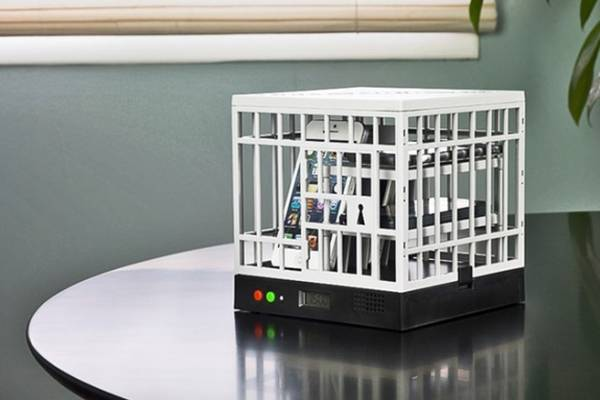
\includegraphics[width=0.35\linewidth]{ReglasBasicas/CajaFuerteCeluar.jpg}
\end{center}
\end{block}
\end{itemize}
\end{frame}

\begin{frame}
\frametitle{Pase de Lista}
\begin{itemize}
\item Se pasa lista al inicio de la clase. En caso de reincorporaci\'on tard\'ia, se pone un retardo.
\item DOS RETARDOS equivalen a una INASISTENCIA, que no es JUSTIFICABLE.
\end{itemize}
\end{frame}


\begin{frame}
\frametitle{Pase de Lista}
Para justificar una inasistencia, es necesario cumplir con los siguientes pasos:
\begin{itemize}	 
\item Ingresar al apartado de Google classroom creado para dicho fin y cargar un archivo PDF. 
\item Agregar un PDF cuyo nombre debe 
iti-$<$clavegrupo$>$-$<$apat$>$-$<$amat$>$-$<$nombre$>$-$<$dd1$>$-$<$mm1$>$-$<$yyyy1$>$-$<$dd2$>$-$<$mm2$>$-$<$yyyy2$>$.pdf
\item Donde dd1,mm1 y yyyy1 es la fecha de inicio inasistencia (si es un solo dia, puede ser 02-09-2024-02-09-2024)
dd2,mm2 y yyyy2 es la fecha de inicio fin de su inasistencia (si falto una semana, puede poner 02-09-2024-06-09-2024)
\item El interior de ese PDF debe contener documento que justifique su inasistencia. \textbf{Solo se reciben inasistencias por motivos medicos y de trabajo (SAT, Pasaporte, VISA, entrevista de trabajo))}. Los motivos meramente personales quedan cubiertos por el 20\% de faltas que se conviene para el estudiante.  
\item Ejemplos
iti-$<$552244$>$-$<$nuño$>$-$<$maganda$>$-$<$marco-aurelio$>$-$<$02$>$-$<$09$>$-$<$2024$>$-$<$02$>$-$<$10$>$-$<$2024$>$.pdf
\end{itemize}
\end{frame}


\begin{frame}
\frametitle{Alumnos con Empleo (1)}
\begin{itemize}
\item Al NO alcanzar un 80\% de asistencia, el estudiante pierde su derecho de ser EVALUADO
\end{itemize}
\begin{block}{Alumnos VIPs}
En caso de tener un empleo formal dentro o fuera de la ciudad, es necesario entregar una \textbf{constancia laboral} que acredite el horario que se esta cubriendo (en el caso de locales, este horario se debe empalmar con el de la materia). En esa constancia debe acreditar que se esta haciendo labores de manera presencial en tal ubicacion. Esto lo dispensa solo del requisito de las asistencias, mas no de los proyectos que deban entregarse. Incluso pudiera solicitarle presentar avance de manera ``remota'' durante alguna de las clases. Enviar esa constancia con copia para el director de carrera.
\end{block}
\end{frame}


\begin{frame}
\frametitle{Alumnos con Empleo (2)}
\begin{itemize}
\item La justificacion de inasistencias por \textit{actividad laboral} se considerar\'a a partir del momento de la recepci\'on de dicha constancia en el correo del instructor (y no a partir de la fecha indicada en la constancia), por lo que si se recibe de manera tardia (con mas de una semana de retardo), dichas inasistencias NO SERAN justificadas.
\item La justificación será válida si el estudiante programa \textbf{POR LO MENOS} dos asesorías por semana. De no hacerlo, pierde el beneficio de la justificación y se aplican las reglas anteriormente establecidas. 
\end{itemize}

\end{frame}











\begin{frame}

\frametitle{Unidades }

\begin{enumerate}
\item Manejo de Errores y Excepciones
\begin{enumerate}
\item Errores y Excepciones
\item Manejo de Errores y Excepciones
\end{enumerate}
\item Manejo de Objetos Gráficos
\begin{enumerate}
\item Componentes Gráficos
\item Librerías
\item Manejo de Eventos
\end{enumerate}
\item Concurrencia
\begin{enumerate}
\item Hilos
\item Concurrencia y Sincronización
\end{enumerate}
\item Programación para Red
\begin{enumerate}
\item Sockets
\item Conexión a Base de Datos
\end{enumerate}

\end{enumerate}

\end{frame}


%------------------------------------------------
\section{Evaluación}
%------------------------------------------------

\begin{frame}
\frametitle{Evaluación (1)}
\begin{itemize}
\item Para cada unidad del curso, se consideran 3 aspectos:
\begin{itemize}
\item Ejercicios o investigaciones especiales (1)- 25\%
\item Proyecto Individual  - 35\%
\item Proyecto en Equipo - 40\%
\end{itemize}
\item Para aprobar el curso, es obligatorio:
\begin{itemize} 
\item Tener calificacion aprobatoria en todas las unidades (100-100-40 no da calificación aprobatoria).
\item Tener por lo menos dos asesorías por semana (Registrarlas por semana, no 30 asesorías al final del cuatrimestre)
\item Cumplir con el 80\% de asistencia mínimo, incluyendo aquellas inasistencias justificadas debidamente
\end{itemize}
\end{itemize}
\end{frame}

\begin{frame}
\frametitle{Evaluación (2)}
Para cada unidad, habra sesiones de ``teoria'', sesiones de seguimiento de proyectos y sesiones de esparci  miento
\begin{itemize}
\item En las sesiones de teoria, el profesor presentara uno o varios temas
\item En las sesiones de seguimiento de proyectos, de manera aleatoria se nombrara al integrante de equipo individual o en equipo. En el caso de que un integrante individual no responda, se le bajarán 5 puntos a su calificación del proyecto
\item En las sesiones de esparcimiento, se permitirá a los estudiantes trabajar en proyectos pendientes, pero se contabilizará la asistencia. 
\end{itemize}
\end{frame}

\begin{frame}
\frametitle{Evaluación (3)}
Sesiones de Seguimento de proyectos
\begin{itemize}
\item En el caso de que el integrante del equipo seleccionado aleatoriamente no responda satisfactoriamente lo cuestionado, se le bajaran 5 puntos a su calificacion del proyecto a todos los integrantes del equipo
\item En el caso de los proyectos en equipo, el integrante seleccionado es aleatorio. Si en una primera ronda le toco al integrante A, en una segunda ronda posiblemente le toque al integrante B
\end{itemize}
\end{frame}



\begin{frame}
\frametitle{Evaluación (4)}
Lo que se debe presentar en una sesion de seguimiento de proyectos
\begin{itemize}
\item En un trabajo individual
\begin{itemize}
\item Compartir pantalla de la ejecucion del avance del proyecto
\item Explicar con recursos multimedia los pasos para la resolucion del proyecto
\item Establecer el avance desde la ultima entrega
\end{itemize}
\item En un trabajo grupal
\begin{itemize}
\item Compartir pantalla de la ejecucion del avance del proyecto
\item Explicar con recursos multimedia los pasos para la resolucion del proyecto
\item Desglosar como se repartio el trabajo entre los integrantes del equipo
\item Establecer el avance desde la ultima entrega
\end{itemize}
\end{itemize}
\end{frame}



\begin{frame}
\frametitle{Evaluación (5)}
Acerca de los proyectos
\begin{itemize}
\item Aleatorios y DIFERENTES para la mayoria (preferentemente para cada integrante)
\item Equipos: Proyectos diferentes para cada equipo, e Integrantes de los mismos formados de manera ALEATORIA!!
\end{itemize}
\end{frame}



\begin{frame}
\frametitle{Fragmentaci\'on de equipos}
\begin{itemize}
\item Si llegar a ocurrir que en un proyecto en equipo no hay un acuerdo para trabajar en equipo (Hay dos o mas entregas del proyecto asignado por partes diferentes dentro del mismo equipo)
\begin{block}{Penalizaci\'on}
Cada ``fragmento'' de equipo recibe una penalizacion de 25 puntos mas las penalizaciones acumuladas por otros rubros. 
\end{block}
\item esta regla \textbf{NO APLICA} cuando hay uno o varios ``desertores'' del equipo (y hay una sola entrega del proyectos en equipo)
\end{itemize}

\end{frame}



\begin{frame}
\frametitle{Acerca de Excensión}
\begin{itemize}
\item Cúando el profesor realizar alguna mecánica para excentar un proyecto (Individual/Equipo/Asignación especial) y uno o varios estudiantes completan lo solicitado, existen dos posibilidades:
\begin{itemize}
\item El estudiante acepta excentar la elaboración de dicho proyecto o actividad, pero al hacer esto asume que la calificación asignada es 70.
\item El estudiante decide hacer el proyecto a pesar de haber excentado. En este caso el estudiante se hace acreedor a 20 puntos que puede aplicar sobre la calificación de dicho proyecto. 

\end{itemize}
\end{itemize}


\end{frame}



%\begin{frame}
%\frametitle{Evaluación (6)}
%Acerca de la participacion
%\begin{itemize}
%\item Se selecciona al azar un estudiante, existen varias posibilidades:
%\begin{itemize}
%\item Esta presente, puede abrir camara, microfono y compartir escritorio para responder lo solicitado, y responde   $\rightarrow$  POSITIVA
%\item Esta presente, NO puede abrir camara, ni microfono, y no comparte escritorio lo solicitado, no es necesario que responda  $\rightarrow$ NEGATIVA
%\item Esta presente, pero decide no participar $\rightarrow$ NEGATIVA
%\item NO esta presente $\rightarrow$ NEGATIVA
%\end{itemize}
%\item La calificacion de Participación es proporcional al porcentaje de participaciones positivas (7/10, 3/5, 0/4, 3/3). 
%\end{itemize}
%\end{frame}




\begin{frame}
\frametitle{Cartucho de Recuperación (REC)}
\begin{itemize}
\item Estudiante tiene derecho a solicitar un ÚNICO proyecto de recuperación aplicable a un solo proyecto o actividad.
\item Esta solicitud debe HACERLA es estudiante - El profesor NO ES RESPONSABLE de informar al estudiante cuando tiene un ADEUDO.  
\item Si el proyecto no entregado es individual, se asigna otro proyecto diferente.
\item Si el proyecto es en equipo, de común acuerdo con los integrantes pueden trabajar en otro proyecto diferente en equipo, o recibir una asignación individual de un proyecto diferente.
\item La calificación recuperada será asignada siempre y cuando cumpla con el porcentaje de falta mínimo necesario para aprobar. Además, debe haber agendado el \% de asesorías proporcional al tiempo de cuatrimestre transcurrido. 
\item El nuevo proyecto asignado esta diseñado para que el estudiante invierta en él por lo menos 1 SEMANA. Si lo solicita un día antes de terminar el cuatrimestre, posiblemente no tendrá tiempo de llevarlo a cabo. 
\end{itemize}
\end{frame}





%------------------------------------------------
\section{Entregables}
%------------------------------------------------



\begin{frame}
\frametitle{Reporte Técnico de Desarrollo de Práctica}
\begin{itemize}
\item Para cada práctica realizada, entregar un documento (\textbf{únicamente en formato PDF*}) con las siguientes secciones:
\begin{itemize}
\item Introducción
\item Desarrollo Experimental
\item Resultados
\item Conclusiones
\item \textbf{Referencias}
\end{itemize}
\item Para GENERAR este reporte es necesario utilizar la plantilla en LATEX (\textbf{únicamente usando LATEX*}) localizada en el siguiente enlace:
\url{https://www.overleaf.com/read/dgkhvfwnygvc}
\end{itemize}
\end{frame}

\begin{frame}
\frametitle{Reporte Técnico de Desarrollo de Práctica}
\begin{itemize}
\item Bajo ninguna circunstancia deben incluir \textbf{CÓDIGO FUENTE}. Si pueden incluir diagrama de flujo, Pseudocódigo, Diagrama E-R, Diagrama de Clases, de Casos de USO, etc. De incluir código fuente, solo tendrá un 50\% del valor en la calificación. 
\item En caso de trabajos indivudales o en EQUIPO, deben emplear la plantilla LaTex que se provee. En caso de utilizar algo diferente a LaTex u otra plantilla de LaTex, la calificación proporcional del informe será \textbf{DESESTIMADA}. 
\item En caso de trabajos en equipo, se debe agregar los integrantes al inicio del INFORME. \textbf{El trabajo solo cuenta para aquellos integrantes mencionados en el informe (y que dicho nombre se encuentre registrado tal cual en la lista). Una vez ENTREGADO, si hay OMISIONES de los integrantes, no se realizará CORRECCION alguna, se debe asumir la consecuencias que esto conlleva. }
\end{itemize}

\end{frame}


\begin{frame}
\frametitle{Ponderación del Informe en la Calificación del Proyecto}
\begin{itemize}
\item Informe: 34 Puntos
\begin{itemize}
\item Uso adecuado de Latex: 5 Puntos
\item Organizaci\'on y Redacci\'on: 6 Puntos
\item Referencias en formato adecuado: 8 Puntos
\item Evidencia del trabajo realizado: 8 Puntos
\item Sin faltas de ortografía ni errores de dedo: 7 Puntos
\end{itemize}
\item Proyecto: 66 Puntos
\begin{itemize}
\item Ejecución y Funcionalidad: 45 Puntos
\item Modularidad: 13 Puntos
\item Documentación: 8 Puntos
\end{itemize}
\end{itemize}
\end{frame}

%------------------------------------------------


% Actualizacion 
%\begin{frame}
%\frametitle{Entregables de proyecto individual}

%\begin{itemize}
%\item \textbf{Clave de GRUPO (incluir guión medio)}
%\item \textbf{Nombre del integrante iniciando por apellido paterno, SIN ESPACIOS y separado por guion bajo}
%\item \textit{\clavegrupo}\_nuno\_maganda\_marco\_aurelio.zip,  \textit{\clavegrupo}\_nuno\_maganda\_marco\_aurelio.pdf, etc. 
%\end{itemize}
%\textbf{Clave de GRUPO seguido del nombre del integrante iniciando por apellido paterno, SIN ESPACIOS y separado por guion bajo}. 
%\begin{itemize}
%\item A su respectiva carpeta de github, cargar lo siguiente:
%\begin{enumerate}
%\item Archivo .ZIP con el código fuente.
%\item Archivo instalador de la aplicación (.APK).  
%\item Archivo PDF con el informe. 
%\end{enumerate}
%\item Mismo formato de NOMBRE de archivo del ENTREGABLE principal para el nombre de los archivos al interior del ZIP
%\end{itemize}

%\end{frame}


\begin{frame}
\frametitle{Entregables de proyecto individual (1)}
    \begin{itemize}
    \item Crear un archivo ZIP con el siguiente formato de nombre:
    \begin{itemize}
        \item \textbf{\clavegrupo\_uX\_nuno\_maganda\_marco\_aurelio}
    \end{itemize}
    \item Dentro, debe contener lo siguiente:
        \begin{itemize}
        \item \textbf{\clavegrupo\_uX\_nuno\_maganda\_marco\_aurelio\_source} (Carpeta con c\'odigo fuente de la aplicaci\'on)
        \item \textbf{\clavegrupo\_uX\_nuno\_maganda\_marco\_aurelio\_latex} (Carpeta con c\'odigo fuente del informe)
        \item \textbf{\clavegrupo\_uX\_nuno\_maganda\_marco\_aurelio.apk} (Instalable (solo si se trata de una aplicación móvil) )
        \item \textbf{\clavegrupo\_uX\_nuno\_maganda\_marco\_aurelio.pdf} (Informe)
        \end{itemize}
    \item Donde:
        \begin{itemize}
        \item \textbf{X} es el n\'umero de unidad a un d\'igito (1, 2, etc)
        \item \textbf{Sustituir con sus apellidos y nombres de manera apropiada} 
        \end{itemize}
    \end{itemize}
%\textbf{Cuatro cuatrimestres ignorando estas instrucciones, ya deber\'ia poner nombres y apellidos. El que lo haga ser\'an sentadillas o p\'aginas, ustedes escojan!}
\end{frame}


\begin{frame}
\frametitle{Entregables de proyecto individual (2)}
    \begin{itemize}
    \item En el caso que un proyecto individual sea asignado en equipo a varios estudiantes, el archivo entregable DEBE MANEJARSE como la de un proyecto individual
    \begin{itemize}
        \item Solo un integrante del equipo carga en la plataforma el entregable individual.
        \item El informe debe llevar los nombres de los integrantes del equipo que trabajaron (Si se omite a alguien, se asume que no trabajo en el proyecto).
		\item NO ES NECESARIO que los otros integrantes marquen en el sistema la tarea como entregada, ya que se conoce su situación desde que se asigna el proyecto. El profesor ya sabe que ustedes van en equipo con el estudiante que hizo la entrega, y por eso deben asegurarse que en el informe entregado, vayan anotados sus nombres.
    \end{itemize}
    \end{itemize}
\end{frame}




\begin{frame}
\frametitle{Entregables de proyectos en equipo}
    \begin{itemize}
    \item Crear un archivo ZIP con el siguiente formato de nombre:
    \begin{itemize}
        \item \textbf{\clavegrupo\_eq\_NN\_uX}
    \end{itemize}
    \item Dentro, debe contener lo siguiente:
%\begin{itemize}
%\item \textbf{Clave de GRUPO (incluir guión)}
%\item \textbf{Palabra equipo seguido del numero de equipo (usando dos digitos)}
%\item Por ejemplo: \textbf{\clavegrupo\_equipo\_01.zip} 
%\end{itemize}
%El contenido del archivo debe ser:
\begin{itemize}
\item \textbf{\clavegrupo\_eq\_NN\_uX\_source} (Carpeta con c\'odigo fuente de la aplicaci\'on)
\item \textbf{\clavegrupo\_eq\_NN\_uX\_latex} (Carpeta con c\'odigo fuente del informe)
%\item \textbf{\clavegrupo\_eq\_NN\_uX.apk} (Instalable - Solo aplicaciones móviles)
\item \textbf{\clavegrupo\_eq\_NN\_uX.pdf} (Informe)
\end{itemize}
Donde:
\begin{itemize}
\item \textbf{NN} es el n\'umero de equipo a dos d\'igitos (01, 02, etc)
\item \textbf{X} es el n\'umero de unidad a un d\'igito (1, 2, etc)
\end{itemize}
\item En cada entrega, \textbf{UN SOLO INTEGRANTE DEL EQUIPO} deberá cargar los siguientes archivos en la carpeta asignada por Github para trabajar
\end{itemize}


%Ejemplos: \textit{claveGrupo}\_equipo\_01.zip, iti-27798\_equipo\_01.pdf, etc
\end{frame}




\begin{frame}
\frametitle{Entregables de asignaciones especiales}
    \begin{itemize}
    \item Crear un archivo ZIP con el siguiente formato de nombre:
    \begin{itemize}
        \item \textbf{\clavegrupo\_aeX\_uY\_nuno\_maganda\_marco\_aurelio}
    \end{itemize}
    \item Dentro, debe contener lo siguiente:
        \begin{itemize}
        \item \textbf{\clavegrupo\_aeX\_uY\_nuno\_maganda\_marco\_aurelio\_source} (Carpeta con c\'odigo fuente de la aplicaci\'on - Cuando aplique)
        \item \textbf{\clavegrupo\_aeX\_uY\_nuno\_maganda\_marco\_aurelio\_latex} (Carpeta con c\'odigo fuente del informe o diapositivas)
        \item \textbf{\clavegrupo\_aeX\_uY\_nuno\_maganda\_marco\_aurelio.apk} (Instalable - Solo aplicaciones móviles)
        \item \textbf{\clavegrupo\_aeX\_uY\_nuno\_maganda\_marco\_aurelio.pdf} (Informe)
        \end{itemize}
    \item Donde:
        \begin{itemize}
        \item \textbf{X} es el n\'umero de asignación dentro de la unidad a un d\'igito (1, 2, etc)
        \item \textbf{Y} es el n\'umero de unidad a un d\'igito (1, 2, etc)
        \item \textbf{Sustituir con sus apellidos y nombres de manera apropiada} 
        \end{itemize}
    \end{itemize}
%\textbf{Cuatro cuatrimestres ignorando estas instrucciones, ya deber\'ia poner nombres y apellidos. El que lo haga ser\'an sentadillas o p\'aginas, ustedes escojan!}
\end{frame}





\begin{frame}
\frametitle{Nombres de Archivos Entregables}
En el caso de nombres y apellidos acentuados, con dieresis o con virgulilla (\textasciitilde{}), sustituir de acuerdo con las siguientes reglas:
\begin{itemize}
\item Sustituir N/n por \~N/\~n
\item Sustituir A/a por \'A/\'a
\item Sustituir E/e por \'E/\'e
\item Sustituir I/i por \'I/\'i
\item Sustituir O/o por \'O/\'o
\item Sustituir U/u por \'U/\'u
\item Sustituir U/u por \"U/\"u
\end{itemize}
\end{frame}



\begin{frame}
\frametitle{Penalizaciones por Entregas Incompletas}
\begin{columns}
\begin{column}{0.5\textwidth}
\begin{itemize}
\item Proyecto que no este entregado de acuerdo con las especificaciones, ser\'a penalizado. Dos escenarios posibles:
\begin{itemize}
\item El proyecto puede revisarse (completo o con faltas al formato).
\item El proyecto NO puede revisarse (falta codigo fuente, informe, APK, no se compila por alguna falla, etc). En automático el proyecto queda descartado.
\end{itemize}
\end{itemize}
\end{column}
\begin{column}{0.5\textwidth}
Se recomienda LEER con cuidado la secci\'on de entregables de esta presentación. Las penalizaciones son acumulables. 
%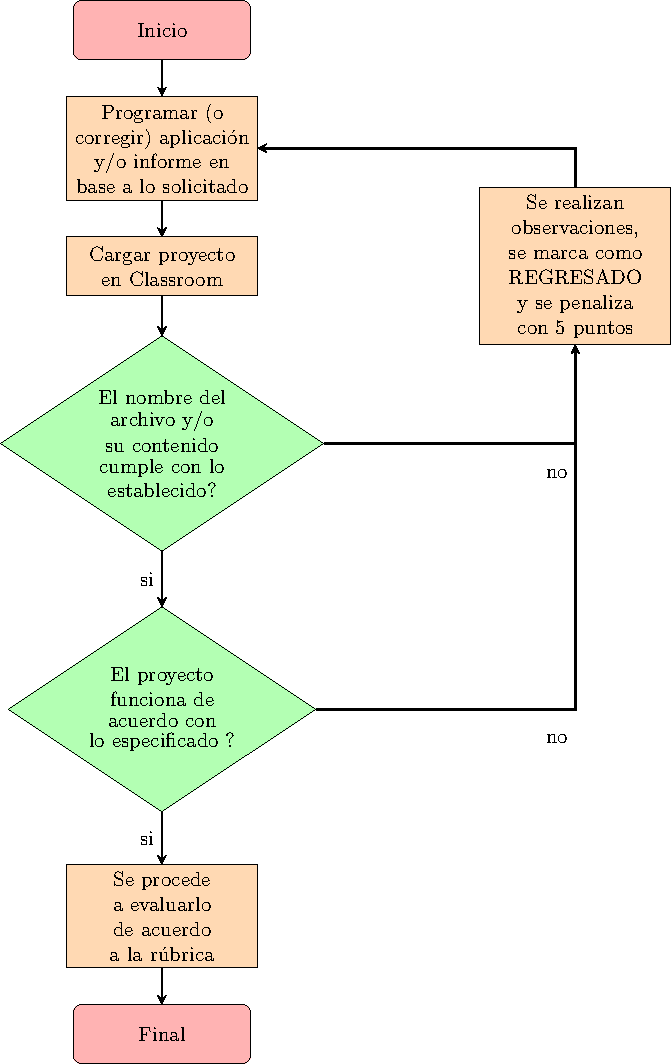
\includegraphics[width=4cm]{DiagramaFlujoVaginal/DF.pdf}
\begin{tabular}{p{3cm}|c}
\hline
\textbf{Falta} & \textbf{Penalizacion} \\
\hline
Nombre Archivo & 8 \\
Tipo de Archivo & 7 \\
Estructura de Directorios  & 6 \\
Falta o Error en Script  & 6 \\
Poner ZIPs dentro del ZIP  & 8 \\
\hline
\end{tabular}
\end{column}
\end{columns}
\end{frame}


\begin{frame}
\frametitle{Salon de la Fama de Entregas Completas e Incompletas}
\begin{columns}
\begin{column}{0.5\textwidth}
\begin{center}
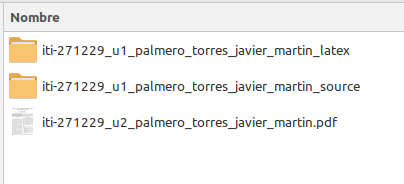
\includegraphics[width=4cm]{Entregables/CasoBien.png}

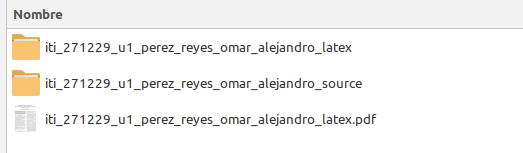
\includegraphics[width=5cm]{Entregables/CasoBien2.png}
\end{center}

\end{column}
\begin{column}{0.5\textwidth}
\begin{center}
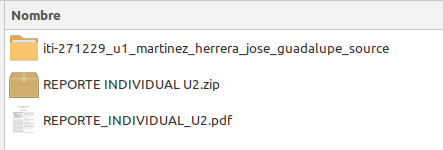
\includegraphics[width=4cm]{Entregables/CasoMal1.png}

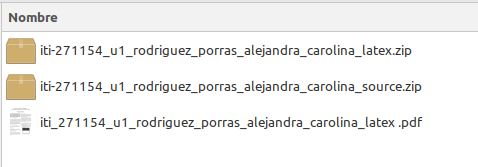
\includegraphics[width=5cm]{Entregables/CasoMal2.png}
\end{center}

\end{column}
\end{columns}
\end{frame}



\begin{frame}
\frametitle{Premio a la Compresión Lectora 2024}
\begin{center}
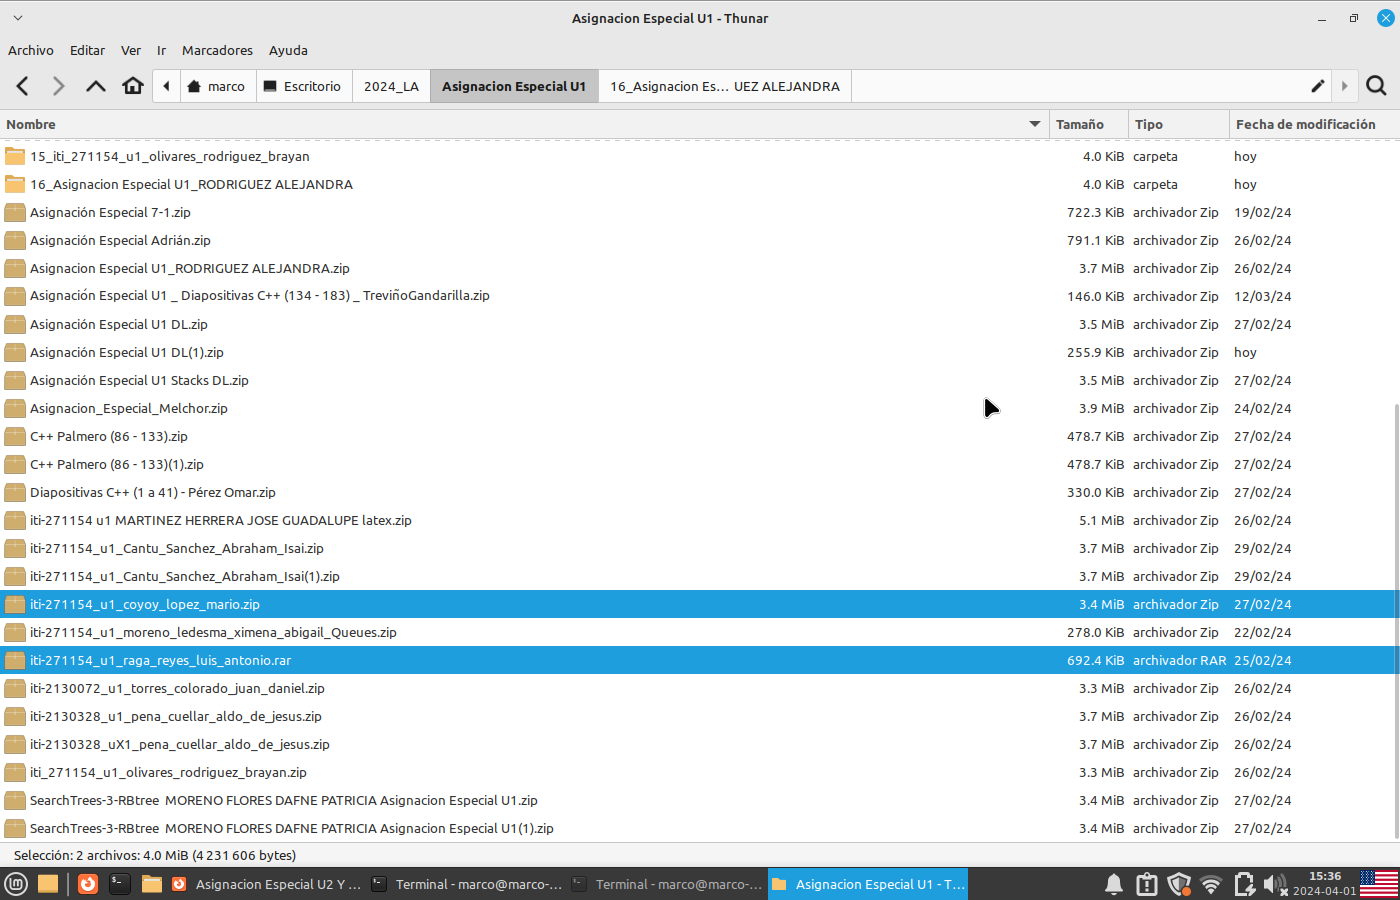
\includegraphics[width=0.75\linewidth]{Entregables/PremioAlaComprensionLectora_2024.png}
\end{center}

\end{frame}







\begin{frame}
\frametitle{Fechas importantes de entrega de proyectos}

\begin{itemize}
\item Fecha de asignación: fecha en que se da a conocer al grupo el trabajo a elaborar
\item Fecha de entrega sin penalización: 14 dias naturales despues de la fecha de asignación
\item Proyecto entregado despues de ha fecha de penalización se le aplica una penalización de 20 PUNTOS
\item Fecha de cierre: 21 días naturales despues de la fecha de asignación. 
\end{itemize}
\begin{block}{Regla ``CANTU''}
\begin{itemize}
\item Ningún proyecto será revisado despues de la fecha de cierre. Se programarán las entregas para cerrar y no permitir entregas tardías. 
\end{itemize}
\end{block}
\end{frame}





\section{Materiales Requeridos}
\begin{frame}
\frametitle{Sistema Operativo Oficial}

\textbf{LINUX}
\begin{block}{En orden de dificultad}
\begin{itemize}
\item Linux instalado de manera emulada usando VirtualBox o VMWare.
\item Crear una USB o HD booteable (con persistencia) y bootear desde su laptop solo para las clases y los proyectos.
\item Linux instalado de manera nativa. Distribuciones recomendadas: \textbf{Mint, Ubuntu, Lubuntu, Xubuntu, Debian}
\end{itemize}
\end{block}
\textbf{** Tienen la opción de no INSTALAR LINUX, pero la evaluación será realiza en una PC con Linux instalado}
\end{frame}


\begin{frame}
\frametitle{Software Utilizado}
Sobre una instalación de Linux, se debe instalar lo siguiente:
\begin{itemize}
\item Navegador Chrome/Firefox actualizado
\item LaTeX para edición de reportes
\item Python3
\item Otras librerias (se espeficarán conforme se vayan utilizando)
\end{itemize}
\end{frame}





\section{Plagio}

\begin{frame}
\frametitle{Plagio}
\Huge
\begin{center}
Se buscan integrantes para ingresar al Salon de la fama del PLAGIO
\end{center}
\end{frame}

\begin{frame}
\frametitle{Plagio}

\begin{columns}[c] % The "c" option specifies centered vertical alignment while the "t" option is used for top vertical alignment
\column{.68\textwidth} % Left column and width
\begin{itemize}
\item Reprobación automática a quien reproduzca códigos de otros compañeros y los reporte como suyos, ademas de una nota en su expediente con copia para el consejo de calidad 
\end{itemize}
\column{.28\textwidth} % Left column and width
\begin{center}

\includegraphics[scale=0.27]{Plagio/tarjeta-roja.jpg}
\end{center}
\end{columns}
\begin{center}
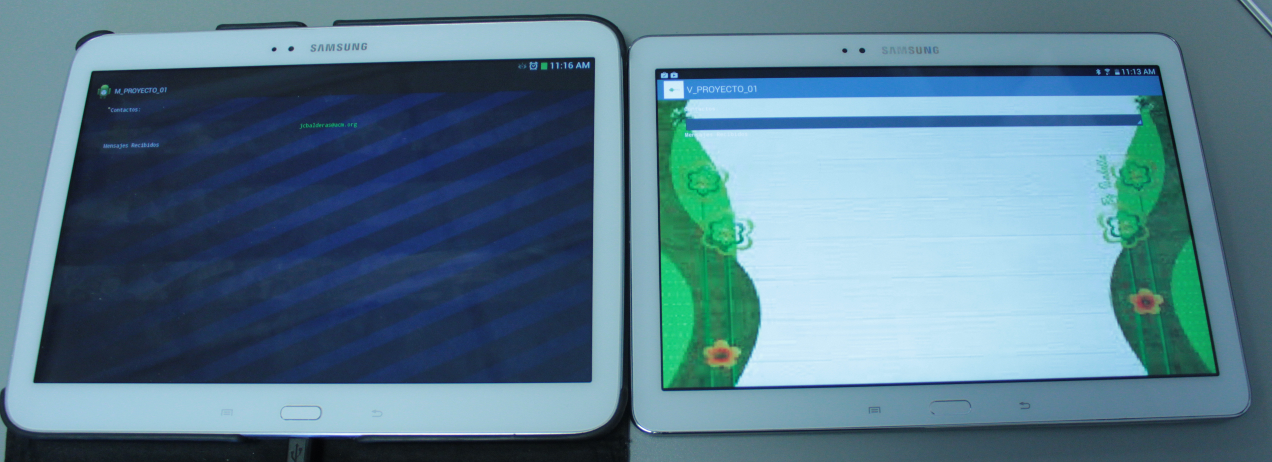
\includegraphics[scale=0.23]{Plagio/Pirata01}
\end{center}
\end{frame}


\begin{frame}
\frametitle{Plagio}
\begin{columns}[c] % The "c" option specifies centered vertical alignment while the "t" option is used for top vertical alignment
\column{.68\textwidth} % Left column and width
\begin{itemize}
\item Reprobación automática a quien copie códigos de Internet y los reporte como suyos, ademas de una nota en su expediente con copia para el consejo de calidad 
\end{itemize}
\column{.28\textwidth} % Left column and width
\begin{center}

\includegraphics[scale=0.27]{Plagio/tarjeta-roja.jpg}
\end{center}
\end{columns}
\begin{center}
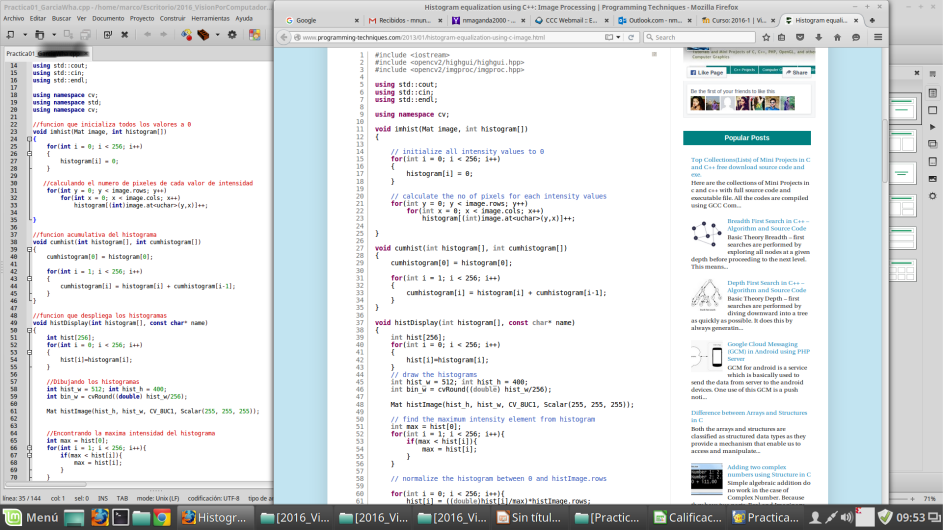
\includegraphics[scale=0.23]{Plagio/Pifia}
\end{center}
\end{frame}

\begin{frame}
\frametitle{Plagio}
\begin{columns}[c] % The "c" option specifies centered vertical alignment while the "t" option is used for top vertical alignment
\column{.68\textwidth} % Left column and width
\begin{itemize}
\item Reprobación automática a quien copie códigos de Internet y los reporte como suyos, ademas de una nota en su expediente con copia para el consejo de calidad 
\end{itemize}
\column{.28\textwidth} % Left column and width
\begin{center}

\includegraphics[scale=0.27]{Plagio/tarjeta-roja.jpg}
\end{center}
\end{columns}
%\url{https://github.com/naman14/AlgorithmVisualizer-Android}
\href{https://github.com/naman14/AlgorithmVisualizer-Android}{https://github.com/naman14/AlgorithmVisualizer-Android}

\begin{columns}[c] % The "c" option specifies centered vertical alignment while the "t" option is used for top vertical alignment
\column{.44\textwidth} % Left column and width
\begin{center}
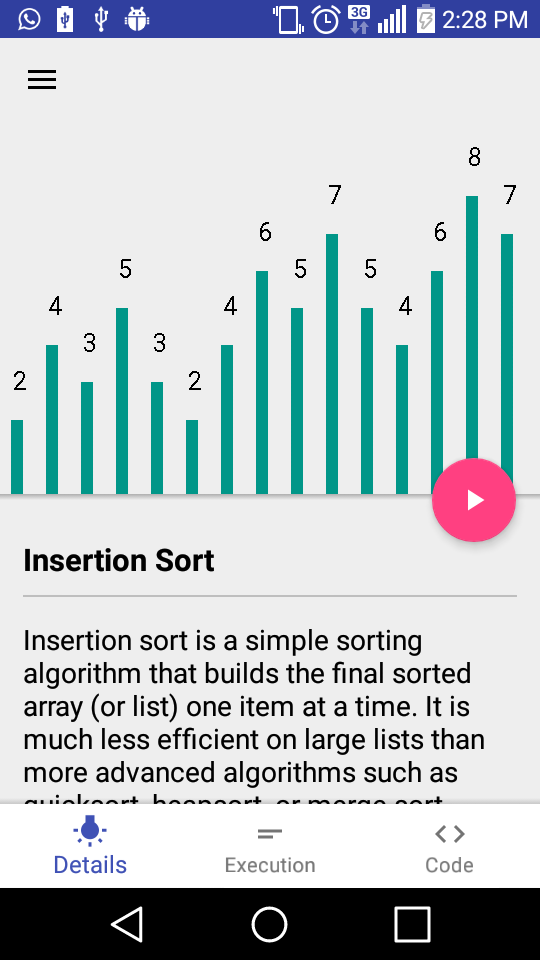
\includegraphics[width=2.3cm]{Plagio/Piratazo_Orig1}\hspace{0.05cm}
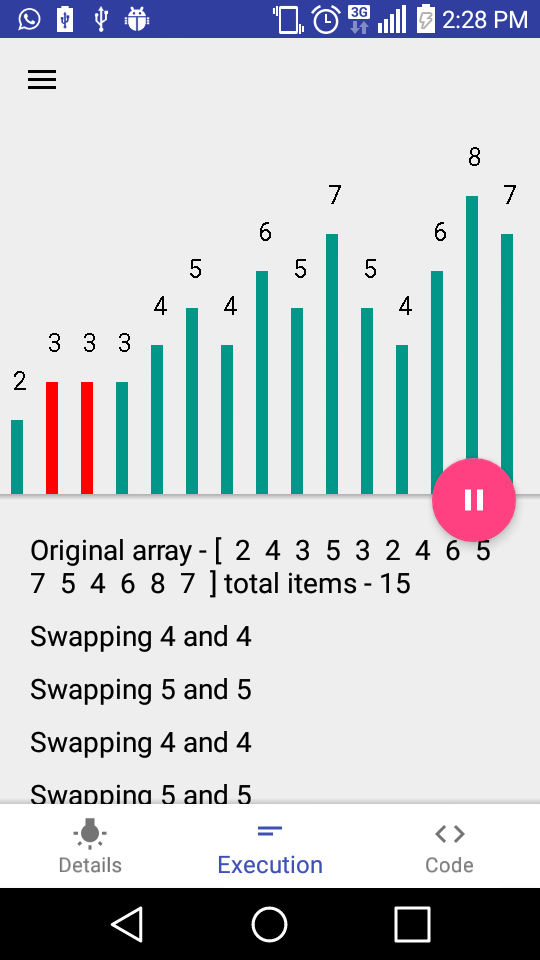
\includegraphics[width=2.3cm]{Plagio/Piratazo_Orig2}\\
Proyecto Original
\end{center}
\column{.44\textwidth} % Left column and width
\begin{center}
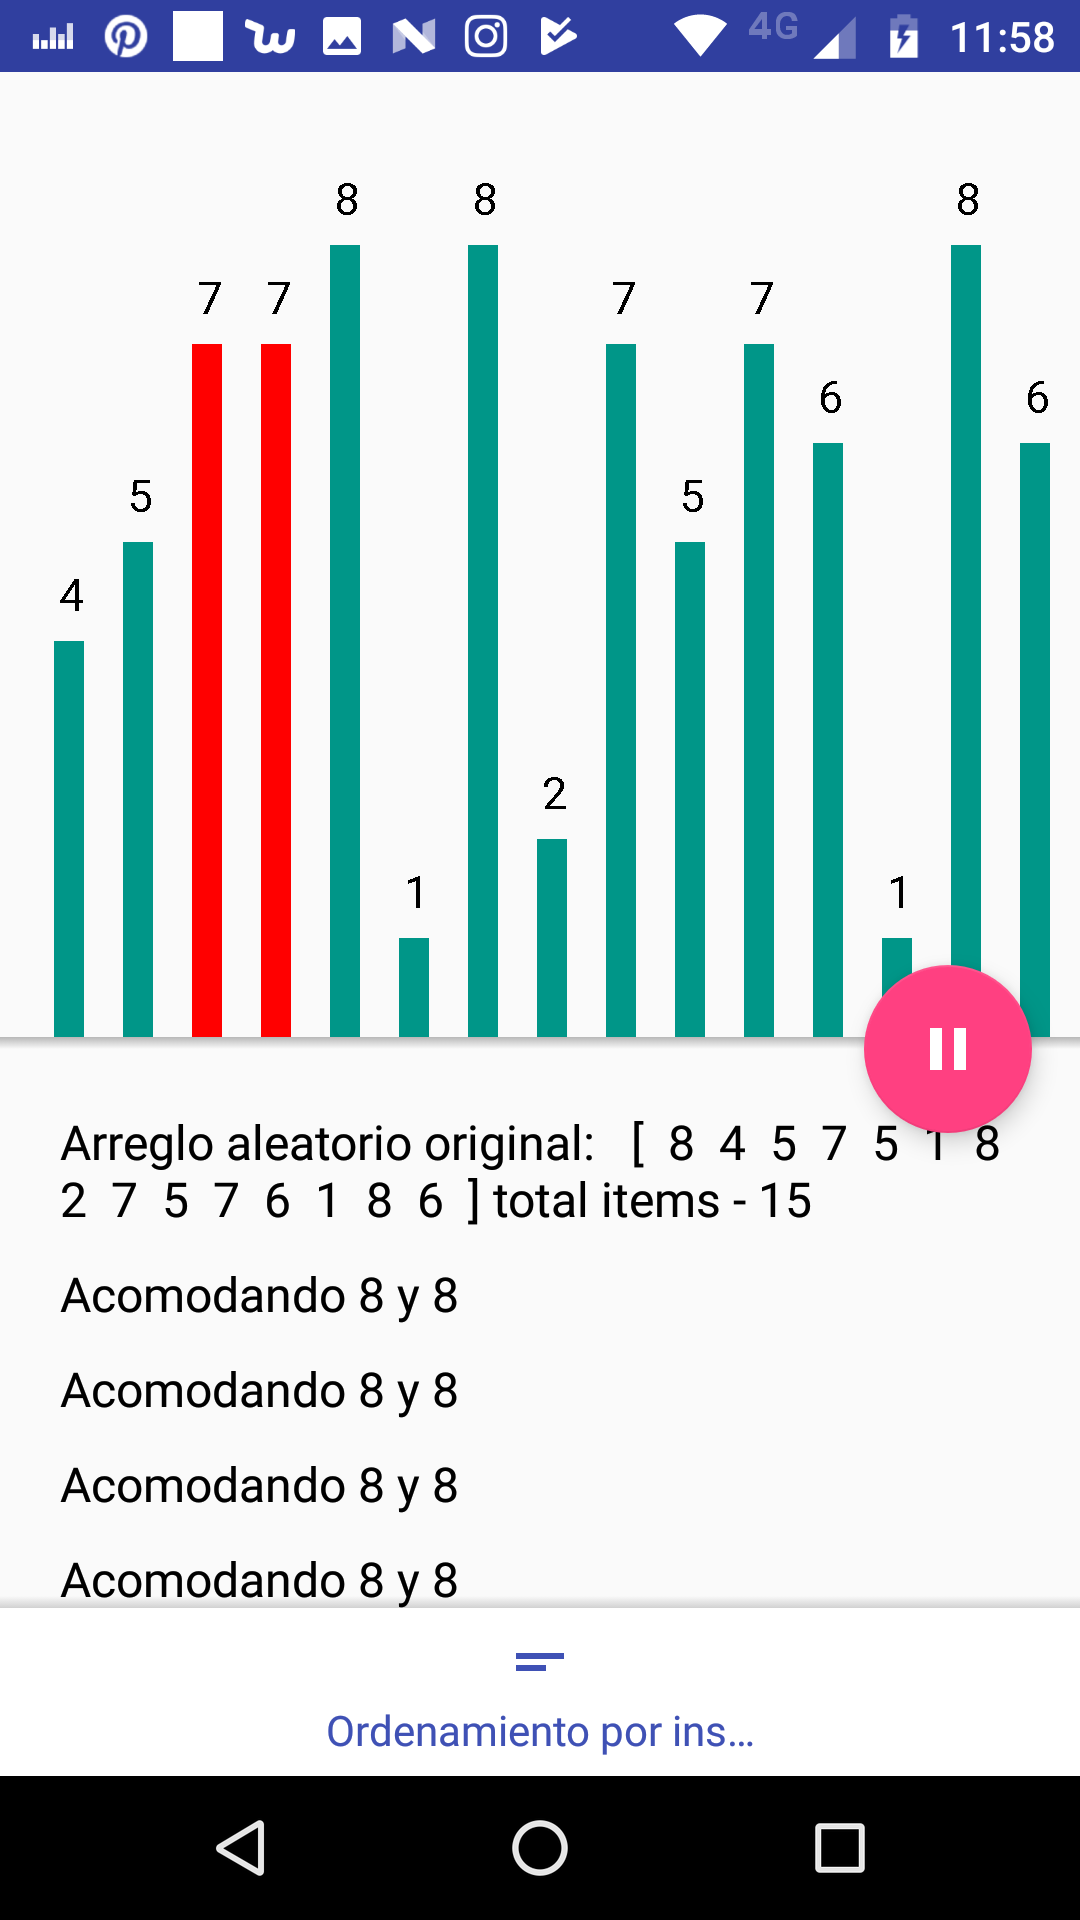
\includegraphics[width=2.3cm]{Plagio/Piratazo_Oscar1}\hspace{0.05cm}
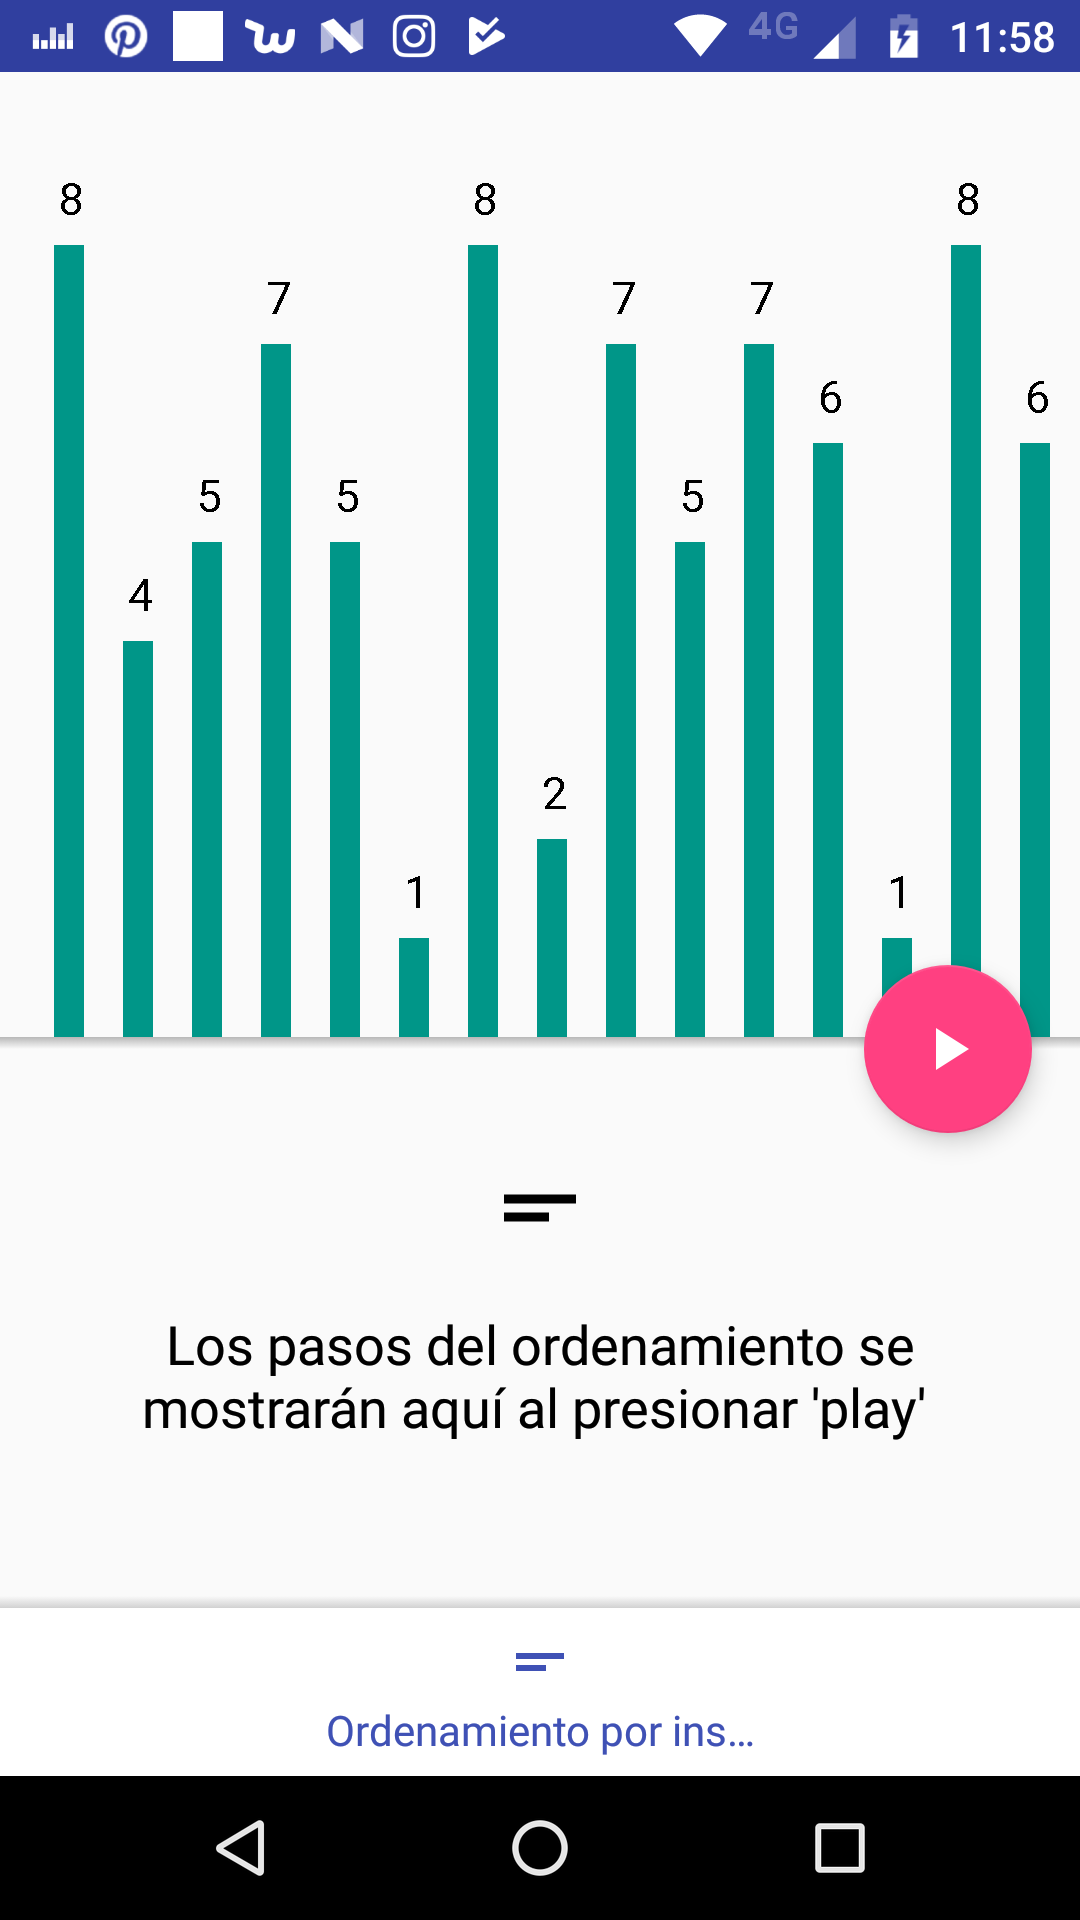
\includegraphics[width=2.3cm]{Plagio/Piratazo_Oscar2}\\
Proyecto ``clonado''
\end{center}	
\end{columns}
\end{frame}





\begin{frame}
\frametitle{Frase célebre}
``Finalmente son jóvenes que están en la preparatoria y que deben de leer su convocatoria con toda claridad, si no cumplen con los requisitos, si no pueden leer una convocatoria que dice tienes que traer número uno esto, número dos esto, número tres esto, no están listos para ser \textbf{estudiantes de educación superior}, así lo digo con toda claridad''.

Sara Ladrón de Guevara.

Rectora de la Universidad Veracruzana (2013-2017 y 2017-2021).

\end{frame}





\begin{frame}
\frametitle{CONCLUSIÓN}
\begin{center}

\includegraphics[scale=0.31]{Conclusion/UNO}
\end{center}
\end{frame}




\end{document}



